%%%% ijcai16.tex

\typeout{Constructive Preference Elicitation by Setwise Max-margin Learning}

\documentclass{article}
\usepackage{ijcai16}
\usepackage{times}
%\usepackage{latexsym}
\usepackage{graphicx}

\RequirePackage{amsmath,amssymb,amsfonts,amsthm}
\usepackage{algorithm}
\usepackage{algpseudocode}

% ---------------------------------------------------------------------------

\algrenewcommand{\algorithmicrequire}{\textbf{Input:}}
\algrenewcommand{\algorithmicensure}{\textbf{Output:}}

\renewcommand\[{\begin{equation}}
\renewcommand\]{\end{equation}}

% Bold math symbols
\newcommand{\bbA}{\mathbb{A}}
\newcommand{\bbB}{\mathbb{B}}
\newcommand{\bbC}{\mathbb{C}}
\newcommand{\bbD}{\mathbb{D}}
\newcommand{\bbE}{\mathbb{E}}
\newcommand{\bbF}{\mathbb{F}}
\newcommand{\bbG}{\mathbb{G}}
\newcommand{\bbH}{\mathbb{H}}
\newcommand{\bbI}{\mathbb{I}}
\newcommand{\bbJ}{\mathbb{J}}
\newcommand{\bbK}{\mathbb{K}}
\newcommand{\bbL}{\mathbb{L}}
\newcommand{\bbM}{\mathbb{M}}
\newcommand{\bbN}{\mathbb{N}}
\newcommand{\bbO}{\mathbb{O}}
\newcommand{\bbP}{\mathbb{P}}
\newcommand{\bbQ}{\mathbb{Q}}
\newcommand{\bbR}{\mathbb{R}}
\newcommand{\bbS}{\mathbb{S}}
\newcommand{\bbT}{\mathbb{T}}
\newcommand{\bbU}{\mathbb{U}}
\newcommand{\bbV}{\mathbb{V}}
\newcommand{\bbW}{\mathbb{W}}
\newcommand{\bbX}{\mathbb{X}}
\newcommand{\bbY}{\mathbb{Y}}
\newcommand{\bbZ}{\mathbb{Z}}

% Calligraphic math symbols
\newcommand{\calvar}[1]{\ensuremath{\mathcal{#1}}}
\newcommand{\calA}{\calvar{A}}
\newcommand{\calB}{\calvar{B}}
\newcommand{\calC}{\calvar{C}}
\newcommand{\calD}{\calvar{D}}
\newcommand{\calE}{\calvar{E}}
\newcommand{\calF}{\calvar{F}}
\newcommand{\calG}{\calvar{G}}
\newcommand{\calH}{\calvar{H}}
\newcommand{\calI}{\calvar{I}}
\newcommand{\calJ}{\calvar{J}}
\newcommand{\calK}{\calvar{K}}
\newcommand{\calL}{\calvar{L}}
\newcommand{\calM}{\calvar{M}}
\newcommand{\calN}{\calvar{N}}
\newcommand{\calO}{\calvar{O}}
\newcommand{\calP}{\calvar{P}}
\newcommand{\calQ}{\calvar{Q}}
\newcommand{\calR}{\calvar{R}}
\newcommand{\calS}{\calvar{S}}
\newcommand{\calT}{\calvar{T}}
\newcommand{\calU}{\calvar{U}}
\newcommand{\calV}{\calvar{V}}
\newcommand{\calW}{\calvar{W}}
\newcommand{\calX}{\calvar{X}}
\newcommand{\calY}{\calvar{Y}}
\newcommand{\calZ}{\calvar{Z}}

% Vectors
\newcommand{\vecvar}[1]{\ensuremath{\boldsymbol{#1}}}
\newcommand{\va}{\vecvar{a}}
\newcommand{\vb}{\vecvar{b}}
\newcommand{\vc}{\vecvar{c}}
\newcommand{\vd}{\vecvar{d}}
\newcommand{\ve}{\vecvar{e}}
\newcommand{\vf}{\vecvar{f}}
\newcommand{\vg}{\vecvar{g}}
\newcommand{\vh}{\vecvar{h}}
\newcommand{\vi}{\vecvar{i}}
\newcommand{\vj}{\vecvar{j}}
\newcommand{\vk}{\vecvar{k}}
\newcommand{\vl}{\vecvar{l}}
\newcommand{\vm}{\vecvar{m}}
\newcommand{\vn}{\vecvar{n}}
\newcommand{\vo}{\vecvar{o}}
\newcommand{\vp}{\vecvar{p}}
\newcommand{\vq}{\vecvar{q}}
\newcommand{\vr}{\vecvar{r}}
\newcommand{\vs}{\vecvar{s}}
\newcommand{\vt}{\vecvar{t}}
\newcommand{\vu}{\vecvar{u}}
\newcommand{\vv}{\vecvar{v}}
\newcommand{\vw}{\vecvar{w}}
\newcommand{\vx}{\vecvar{x}}
\newcommand{\vy}{\vecvar{y}}
\newcommand{\vz}{\vecvar{z}}
\newcommand{\valpha}{\vecvar{\alpha}}
\newcommand{\veps}{\vecvar{\varepsilon}}
\newcommand{\vphi}{\vecvar{\varphi}}
\newcommand{\vpsi}{\vecvar{\psi}}
\newcommand{\vtheta}{\vecvar{\theta}}

% Operators
\DeclareMathOperator*{\argmax}{argmax}
\DeclareMathOperator*{\argmin}{argmin}

% Debugging

\usepackage{color}
\newcommand{\andrea}[1]{{\bf \textcolor{blue}{{\fbox{Andrea:} #1}}}}
\newcommand{\stefano}[1]{{\bf \textcolor{green}{{\fbox{Stefano:} #1}}}}
\newcommand{\paolo}[1]{{\bf \textcolor{red}{{\fbox{Paolo:} #1}}}}

% ---------------------------------------------------------------------------

\title{Constructive Preference Elicitation by Setwise Max-margin Learning}
\author{ST and AP and PV}

\begin{document}

\maketitle

\begin{abstract}
WRITEME
\end{abstract}

\section{Introduction}

WRITEME

- importance of recommendation systems and preference elicitation

- existing approaches and their limitations

% constructive preference elicitation
In this paper we take a {\em constructive} view on preference
elicitation, enlarging its scope from the selection of items among a
set of candidates to the synthesis of entirely novel
instances. Instances are represented as combinations of basic elements
(e.g. the components of a laptop) subject to a set of constraints
(e.g. the laptop model determines the set of available CPUs). A
utility function is learned over the feature representation of an
instance, as customary in many preference elicitation approaches. The
recommendation is then made by solving a constrained optimization
problem in the space of feasible instances, guided by the learned
utility. \andrea{other constructive preference elicitation approaches?}

% setwise max-margin formulation to deal with uncertainty in user utility
Learning a user utility function requires setting a preference
elicitation strategy and dealing with uncertain and possibly
inconsistent user feedback. Bayesian preference elicitation approaches
deal with both problems by building a probability distribution on
candidate functions and asking queries maximizing informativeness
measures such as expected value of information (EVOI)~\cite{}. These
approaches are however computationally expensive and cannot scale to
fully constructive scenarios, as shown in our experimental results.
We take a space decomposition perspective and jointly learn a set of
weight vectors, each representing a candidate utility function,
maximizing diversity between the vectors and consistency with the
available feedback. These two conflicting objectives tend to generate
equally plausible alternative hypotheses for the unknown
utility. Preference elicitation works by combining weight vector
learning with instance generation, so that each iteration of the
algorithm produces two outcomes: a set of weight vectors and a set of
instances, each maximizing its score according to one of the weight
vectors. 


- experimental results

- paper structure


\section{Related Work}

WRITEME

\section{Setwise Max-margin Learning}

\stefano{Paolo, feel free to improve the text and especially the citations
as you see fit.}

\paragraph{Notation.} We use boldface letters $\vx$ to indicate vectors, and
calligraphic capital letters $\calX$ for sets. We frequently abbreviate the set
$\{ x^i \}_{i=1}^n$ as $\{ x^i \}$ whenever the range of the index $i$ is clear
from the context, and use $[n]$ as a shorthand for the set $\{1, \ldots, n\}$.
The $\ell_1$ vector norm is denoted by $\|\vx\|_1 := \sum_z |x_z|$.

\paragraph{Setting.} We assume to have a multi-attribute feature space $\calX$
of configurations $\vx = (x_1, \ldots, x_n)$ over $n$ features. For the time
being we will focus on binary features only, i.e. $x_z\in\{0,1\}$, to keep
matters simple. This is a common choice for preference elicitation methods,
e.g.~\cite{guo2010real,viappiani2010optimal}; discrete features are handled by
means of a simple one-hot encoding. Partial support for continuous features
will be discussed later on.

We further assume that the set of {\em feasible} configurations is expressed as
a conjunction of linear constraints. This is not a severe restriction:
arbitrary propositional constraints can be trivially encoded in this setting,
e.g. the ``Boolean disjunction'' of two binary variables $x_1 \lor x_2$ can be
rewritten as $x_1 + x_2 \ge 1$. The full set of feasible configurations is
denoted by $\calX_\text{feasible}$.

In adherence to previous work~\cite{guo2010real,viappiani2010optimal}, we model users by means
of linear utility functions: the user's preferences are represented by a weight
vector $\vw\in\bbR^n$, and the utility of a configuration $\vx$ is given by
$\langle \vw, \vx \rangle = \sum_{z=1}^n w_z x_z$. In the following we
require all weights to be {\em non-negative} and {\em bounded}: the individual
weights $w_z$ must fall in a (constant but otherwise arbitrary) interval
$[w^\bot_z, w^\top_z]$, with $w^\bot_z \ge 0$. Both requirements are quite
natural, and enable the translation of our core optimization problem into a
mixed-integer linear problem (as done in Section~\ref{sec:formulation}).

During learning, the actual weight vector $\vw$ is {\em unknown} to the
learning system, and must be estimated from pairwise choices elicited from the
user. The set of examples consists of pairwise comparisons between a more
preferred configuration $\vy_+$ and a less preferred one $\vy_-$. Each preference
induces a ranking constraint $\langle \vw, \vy_+ - \vy_- \rangle \ge 0$.
Details on the actual query selection strategy will be provided in
Section~\ref{sec:querystrategy}.
\stefano{add indifference}

\subsection{Problem Formulation}
\label{sec:formulation}

\paragraph{Non-linear Formulation.} We now introduce an initial formulation of
the optimization problem, that we do {\em not} aim at solving directly.

In the set-margin approach, the goal is twofold. First, for any given set size
$k\geq 1$, we want to find a {\em set} of $k$ weight vectors $\vw^{1},
\ldots, \vw^{k}$, chosen so that all preferences (examples) are satisfied by
the largest possible margin. This is achieved by translating all binary
preferences into inequalities of the form $\langle \vw^i, \vy^h_+ - \vy^h_- \rangle
\geq M$, where $h$ ranges over the examples, and maximizing the margin $M$.
Non-separable datasets, which occur in practice due to user inconsistency, are
handled by introducing slack variables. The updated constraints look as follows:
%
$$ \langle \vw^{i}, \vy^{h}_+ - \vy^{h}_- \rangle \ge M - \varepsilon^{i}_h $$
%
where $\varepsilon^{i}_h$ is the penalty incurred by weight vector $\vw^{i}$
for violating the ranking of example $h$.

Second, we want to produce a set of $k$ configurations $\vx^{1}, \ldots,
\vx^{k}$, so that each configuration $\vx^{i}$ is the ``best'' possible
option when evaluated according to the corresponding $\vw^{i}$. Ideally,
this requirement would be implemented as:
%
$$ \vx^{i} = \argmax_{\vx \in \calX_\text{feasible}} \langle \vw^{i}, \vx^{i} \rangle $$
%
However this formulation is highly impractical. We therefore only require 
each option $\vx^{i}$ to be the best {\em among} the configurations
$\{ \vx^i \}$. This can be accomplished by imposing
constraints of the form $\langle \vw^{i}, \vx^{i} - \vx^{j} \rangle \geq M$
for all $i,j\in[k]$, $i \ne j$.
This however does not guarantee that the produced $\{ \vx^{i} \}$ have a high
{\em absolute} utility. We therefore favor high-quality configurations by
introducing an additional term $\sum_{i=1}^k \langle \vw^{i}, \vx^{i} \rangle$
in the objective function.

A straightforward encoding of the above desiderata leads to the following {\em
non-linear} optimization problem over the variables $M$, $\{ \vw^i \}$, $\{ \vx^i \}$:
%
{\footnotesize
\begin{align}
    \max
        & \;\; M - \alpha \sum_{i=1}^k \| \veps^{i} \|_1 - \beta \sum_{i=1}^k \| \vw^{i} \|_1 + \gamma \sum_{i=1}^k \langle \vw^{i}, \vx^{i} \rangle
        \nonumber
    \\
    \text{s.t.}
        & \;\; \forall \; i \in [k], \forall \; h \in [n] \nonumber
    \\
        & \;\; \qquad \langle \vw^{i}, \vy^{h}_+ - \vy^{h}_- \rangle \ge M - \varepsilon^{i}_h \label{eq:wyconstr}
    \\
        & \;\; \forall \; i, j \in [k], i \neq j \;.\; \langle \vw^{i}, \vx^{i} - \vx^{j} \rangle \ge M \label{eq:wxconstr}
    \\
        & \;\; \forall \; i \in [k] \;.\; \vw^\bot \le \vw^{i} \le \vw^\top \label{eq:wbounds}
    \\
        & \;\; \forall \; i \in [k] \;.\; \vx^{i} \in \calX_{\text{feasible}} \label{eq:xbounds}
    \\
        & \;\; \forall \; i \in [k] \;.\; \veps^{i} \ge 0 \nonumber
    \\
        & \;\; M \ge 0 \nonumber
\end{align}
}
%
Let us illustrate the above piece by piece. The objective is composed of four
parts: we maximize the shared margin $M$ (first part) and minimize the total
sum of the ranking errors $\veps^i$ incurred by each weight vector $\vw^{i}$
(second part), while at the same time regularizing the magnitude of the
weights (third part) and quality of the configurations $\{ \vx^{i} \}$ (last
part). The non-negative hyperparameters $\alpha,\beta,\gamma$ control the
influence of the various components.

The third part requires requires some further explanation. We choose an
$\ell_1$ regularizer in order to facilitate learning {\em sparse} weight
vectors: it is reasonable to assume that a user will have strong opinions
over some attributes, but will be indifferent over most of them.
\stefano{Andrea, improve the above please}

The two core constraints as Equations~\ref{eq:wyconstr} and \ref{eq:wxconstr},
which are taken directly from the discussion above. The former enforces the
correct ranking of the observed user preferences, while the latter ensures that
the generated configurations are ranked correctly with respect to the
corresponding weight vectors. Equations \ref{eq:wbounds} and \ref{eq:xbounds}
ensure that the weights and configurations are in fact feasible, while the
remaining two guarantee the non-negativity of the slack and margin variables.
Since we require $\vw^\bot \ge 0$, Eq.~\ref{eq:wbounds} also enforces the
weights to be non-negative.

Note that we are choosing the options $\{ \vx^i \}$ and the weight vectors $\{
\vw^i \}$ {\em simultaneously}. Since we maximize the margin $M$, the optimizer
will prefer a set of outcomes $\{ \vx^{i} \}$ that partition the weight space
roughly equally, and corresponding utility functions such that each $\vw^{i}$
lies (intuitively) close to the centre of each subregion. See
Figure~\ref{fig:setmargin} for a depiction of this intuition.

\stefano{for $k=1$, setting $\alpha < 1$  renders the problem unbounded, as
Eq.~\ref{eq:wxconstr} vanishes.}

\begin{figure}[t]
    \begin{center}
        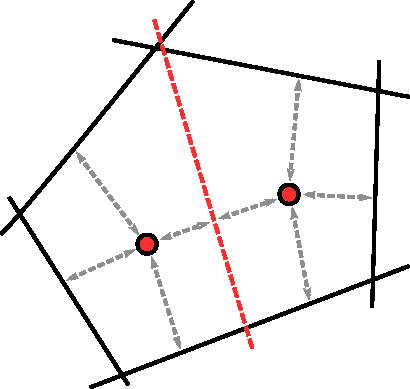
\includegraphics[width=16em]{setmargin}
    \end{center}
    \caption{\label{fig:setmargin} Intuition.}
\end{figure}

\paragraph{MILP Formulation.} This initial formulation is problematic, as
Eq~\ref{eq:wxconstr} involves quadratic terms. Here we show how to reformulate
the problem as a mixed integer linear program (MILP). Our goal is to replace
Eq~\ref{eq:wxconstr} with a set of linear constraints through a suitable
variable transformation.

In order to do so, we introduce a set of fresh variables $p^{i,j}_z$ for every
$i,j\in[k]$ and $z\in[n]$. Assuming for the time being that the new variables
do satisfy the equation $p^{i,j}_z = w^i_z x^i_z$, we rewrite the fourth
component of the objective function in terms of the new variables as:
%
$$ \gamma \sum_{i=1}^k \sum_{z=1}^n p^{i,i}_z $$
%
and, similarly, Eq~\ref{eq:wxconstr} as:
%
\[ \forall \; i, j \in [k], i \neq j \;.\; \sum_{z=1}^n p^{i,i}_z - p^{i,j}_z \ge M \label{eq:pxconstr} \]
%
The fact that $p^{i,j}_z = w^{i}_z x^{i}_z$ is achieved by
setting the following additional constraints. We distinguish between two cases:
(i) $p^{i,i}_z$, and (ii) $p^{i,j}_z$ for $i \ne j$.  Recall that we are
maximizing the margin $M$. Now, due to Eq~\ref{eq:pxconstr}, the optimizer will
try to keep $p^{i,i}_z$ as large as possible and $p^{i,j}_z$ as small as
possible. \stefano{this is not necessarily the case, $M$ is bounded by the
$y$'s as well.}

(Case i) We add an explicit upper bound:
%
$$ p^{i,i}_z \le \min \{ w_\text{max} x^{i}_z, w^{i}_z \} $$
%
where $w_\text{max}$ is a sufficiently large constant.
On one hand, if $x^i_z = 0$ the product $w^i_z x^i_z$ evaluates to $0$, and so does
the upper bound $w_\text{max} x^{i}_z = 0$. On the other hand, if $x^i_z=1$
then the product $w^i_z x^i_z$ amounts to $w^i_z$, while the upper
bound reduces to $\min \{ w_\text{max}, w^{i}_z \}$. By taking a sufficiently
large constant $w_\text{max}$ (e.g. $w_\text{max} := \max_z w^\top_z$) the
upper bound simplifies to $w^i_z$. Since $p^{i,i}_z$ is being maximized, in
both cases it will attain the upper bound, and thus satisfy $p^{i,j}_z = w^i_z x^i_z$.

(Case ii) We add an explicit lower bound:
%
$$ p^{i,j}_z \ge \max \{ 0, w^{i}_z - w_\text{max}(1 - x^{j}_z) \} $$
%
If $x^i_z = 1$ the lower bound simplifies to $\max \{ 0, w^{i}_z \} = w^{i}_z$,
due to the non-negativity of $w^i_z$. Otherwise, if $x^i_z = 0$
then the lower bound becomes $\max \{ 0, w^{i}_z - w_\text{max} \}$, where
the second term is at most $0$. Since $p^{i,j}_z$ is being minimized, in both
cases it will attain the lower bound, and thus satisfy $p^{i,j}_z = w^i_z x^i_z$.

Substituting the above MILP constraints into the original non-linear
formulation, we obtain the following mixed-integer linear problem:
%
{\footnotesize
\begin{align}
    \max
        & \;\; M - \alpha \sum_{i=1}^k \| \veps^{i} \|_1 - \beta \sum_{i=1}^k \| \vw^{i} \|_1 + \gamma \sum_{i=1}^k \sum_{z=1}^n p^{i,i}_z
        \nonumber
    \\
    \text{s.t.}
        & \;\; \forall \; i \in [k], \forall \; h \in [n] \nonumber
    \\
        & \;\; \qquad \langle \vw^{i}, \vy^{h}_+ - \vy^{h}_- \rangle \ge M - \varepsilon^{i}_h \nonumber
    \\
        & \;\; \forall \; i, j \in [k], i \neq j \;.\; \sum_{z=1}^n p^{i,i}_z - p^{i,j}_z \ge M
    \\
        & \;\; \forall \; i \in [k], \forall \; z \in [n] \nonumber
    \\
        & \;\; \qquad p^{i,i}_z \le \min \{ w_\text{max} x^{i}_z, w^{i}_z \}
    \\
        & \;\; \forall \; i, j \in [k], i \neq j \nonumber
    \\
        & \;\; \qquad p^{i,j}_z \ge \max \{ 0, w^{i}_z - w_\text{max}(1 - x^{j}_z) \}
    \\
        & \;\; \forall \; i \in [k] \;.\; \vw^\bot \le \vw^{i} \le \vw^\top \nonumber
    \\
        & \;\; \forall \; i \in [k] \;.\; \vx^{i} \in \calX_{\text{feasible}} \nonumber
    \\
        & \;\; \forall \; i \in [k] \;.\; \veps^{i}_h \ge 0 \nonumber
    \\
        & \;\; M \ge 0 \nonumber
\end{align}
}
%
which can be solved by any suitable MILP solver.

\subsection{Set-wise Preference Elicitation}

\stefano{WRITEME}

See Algorithm~\ref{alg:setmargin}.

\begin{algorithm}
{\footnotesize
\begin{algorithmic}[1]
    \Procedure{SetMargin}{$k, \alpha, \beta, \gamma, T$}
        \State $\calQ \gets \emptyset$
        \For{$t = 1, \ldots, T$}
            \State \{$\vw^{i}, \vx^{i}\}_{i=1}^k \gets \text{{\sc Solve}}(\calQ, k, \alpha, \beta, \gamma)$
            \For{$\vx^{i},\vx^{j} \in \{ \vx^{1}, \ldots, \vx^{k} \} \; \text{{\bf s.t.}} \; i < j$}
                \State $\calQ \gets \calQ \cup \text{{\sc QueryUser}}(\vx^{i},\vx^{j})$
            \EndFor
        \EndFor
        \State $\vw^*, \vx^* \gets \text{{\sc Solve}}(\calQ, 1, \alpha, \beta, \gamma)$
        \State ${\bf return}\; \vw^*, \vx^*$
    \EndProcedure
\end{algorithmic}
}
\caption{\label{alg:setmargin} The {\sc SetMargin} algorithm. Here $k$ is the
set size, $\alpha,\beta,\gamma$ are the hyperparameters, and $T$ is the maximum
number of iterations. The values of $\calX_\text{feasible}$, $\vw^\top$ and
$\vw^\bot$ are left implicit.}
\end{algorithm}

\subsection{Query Strategy}
\label{sec:querystrategy}

\stefano{WRITEME}

The simplest alternative is to query the user $\frac{1}{2}n(n-1)$ pairs.

\paragraph{Generalization to real variables.}

\stefano{WRITEME}

\section{Experiments}
\label{sec:experiments}

In this section we provide extensive experimental evaluation of the {\sc
SetMargin} algorithm. We implemented the {\sc SetMargin} algorithm using
Python, leveraging Gurobi 6.5.0 as the MILP solver. Both the {\sc SetMargin}
source code and the full experimental setup are available at \stefano{add URL}.

We compare {\sc SetMargin} against two strong Bayesian baselines:
\cite{guo2010real} and \cite{viappiani2010optimal}.
\stefano{Paolo, could you describe the baselines?}

We adopted the {\em indifference-augmented} Bradley-Torr user response model
introduced in~\cite{guo2010real}. When queried about a pair of configurations,
the user replies with the true utility of the two items. According to the
classical Bradley-Torr model, which does not attempt to model {\em indifference},
the proabability that a user $\vw$ will prefer configuration $\vx^i$ over
the alternative $\vx^j$, barring indifference, amounts to:
%
$$ (1 + \exp(-\alpha \langle\vw,\vx^i - \vx^j\rangle))^{-1} $$
%
In other words, the probability grows with the difference between the utilities
of the two items. Support for indifference has been introduced
in~\cite{guo2010real} by postulating that the probability of the user being
indifferent about the two configurations $\vx^i, \vx^j$ depends on how close
the two utilities are, as in:
%
$$ \exp(\beta |\langle\vw,\vx^i - \vx^j\rangle|) $$
%
The parameters $\alpha$ and $\beta$ were set as in~\cite{guo2010real}. Please
see the latter for more details
\stefano{The above does not satisfy me at all.}

In all experiments we use an internal 5-fold cross-validation procedure to update the
hyperparameters $\alpha$, $\beta$, and $\gamma$ after every 5 iterations. The
hyperparameters are chosen as to minimize the ranking loss over the user
answers collected so far. $\alpha$ is taken in $\{20, 15, 10, 5, 1\}$,
while $\beta$ and $\gamma$ are taken in $\{10, 5, 1, 0.5, 0.1\}$.
\stefano{explain that we can't turn off $\gamma$}

\paragraph{Synthetic Dataset.} Following the experimental protocol
in~\cite{guo2010real} and \cite{viappiani2010optimal}, in the first experiment
we evaluate the behavior of the proposed method in a challenging artificial
setting. We developed seven synthetic datasets: each dataset involves
$n=2,\ldots,7$ attributes, where each attribute takes one of $n$ possible
values. More explicitly, for $n=2$ the synthetic dataset is
$\calX_\text{feasible} = [2] \times [2]$, for $n=3$ to $\calX_\text{feasible} =
[3] \times [3] \times [3]$, and so on. The cardinality of
$\calX_\text{feasible}$ is $n^n$, and grows (super) exponentially with $n$. For
$n=3$, the dataset is comparable to the synthetic one used
in~\cite{guo2010real} and~\cite{viappiani2010optimal} (which have three domains
of size of 2, 2 and 5, respectively, for a total of 20 feasible
configurations), while for larger $n$ it grows much larger than those typically
used in the Bayesian preference elicitation literature, and as such represents
a good test bed for comparing the scalability of the various methods.
The feasible configuration space was encoded in {\sc SetMargin} through
appropriate MILP constraints, while the other methods required all datasets to
be explicitly grounded.

Users were simulated by drawing random utility vectors from four different
distributions. The first two mimic those used in~\cite{guo2010real}: (1) a
uniform distribution over $[1, 100]$ for each individual weight, and (2) a
normal distribution with mean $25$ and covariance $\frac{25}{3}$\footnote{This
procedure differs from the one reported in~\cite{guo2010real}; we opted for
following the procedure implemented in their code. \stefano{more diplomacy needed}}.
We further produced two novel {\em sparse} sets of weight vectors by deleting
$80\%$ of the entries of the vectors sampled in the uniform and normal settings
uniformly at random \stefano{Paolo, is this correct?}. We sampled $100$
vectors for each setting. All methods were evaluated on the very same weight
vectors.

\stefano{plot average utility loss at the increase of dataset size}

\stefano{plot average runtime at the increase of dataset size}

\stefano{comment on usefulness of sparse weights}

\paragraph{Constructive dataset.} Next, we tested {\sc SetMargin} on a truly
constructive setting. We developed a constructive version of the PC dataset
used in~\cite{guo2010real}: instead of explicitly enumerating all possible PC
item, we definined the set of feasible configurations through MILP constraints.

A PC configurations is defined by seven attributes: computer type (laptop,
desktop, or tower), manufacturer, CPU model, monitor size, RAM amount, storage
size, and price. See Table~\ref{tab:pcdataset} for an overivew of the
attributes. The price attribute is defined as a linear combination of the other
attributes: this is a fair modeling choice, as often the price of a PC is
well approximated by sum of the price of its components plus an offset due to
branding. Compared to the PC dataset in~\cite{guo2010real}, we combined the CPU
type and CPU frequency attributes into a single CPU attribute (e.g. ``PowerPC
G4 @733 MHz''), so to avoid multiplicative terms in the price function.
\stefano{too detailed/handwavy?}

Interactions between attributes are expressed as Horn clauses. An example
costraint might look like this: ``if the manufacturer is Apple, then the
CPU must be either a PowerPC G3 or a PowerPC G4'', which can be encoded
into MILP form as:
%
$$ (1 - x_\text{Apple}) + x_\text{G3} + x_\text{G4} \ge 1 $$
%
Note that mutual exclusivity between all binary variables corresponding to an
attribute ensures that only one of $x_\text{G3}$ and $x_\text{G4}$ can be 1.
The dataset includes constraints between the following attributes: manufacturer
$\to$ type, manufacturer $\to$ CPU, type $\to$ RAM amount, type $\to$ storage
size, type $\to$ monitor size. In total we encoded 16 Horn constraints, each
with one head and multiple options in the body. We do not report the full
list due to space limitations.

\begin{table}
    \centering
    \begin{tabular}{ccc}
        {\bf Attribute} & {\bf Type} & {\bf Values} \\
        \hline \hline
        Type & discrete & 3 \\
        Manufacturer & discrete & 8 \\
        CPU model & discrete & 37 \\
        RAM amount & discrete & 10 \\
        HD size & discrete & 10 \\
        Monitor size & discrete & 8 \\
        Price & continuous & --
    \end{tabular}
    \caption{\label{tab:pcdataset} Statistics for the PC dataset.}
\end{table}

- PC dataset without costs

- PC dataset with costs

\section{Conclusion}

WRITEME

\section*{Acknowledgments}

WRITEME

\bibliographystyle{named}
\bibliography{ijcai16}

\onecolumn

\begin{figure}[b]
    \centering
    \begin{tabular}{cccc}
        {\bf synthetic 2} & {\bf synthetic 3} & {\bf synthetic 4} & {\bf synthetic 5}
        \\
        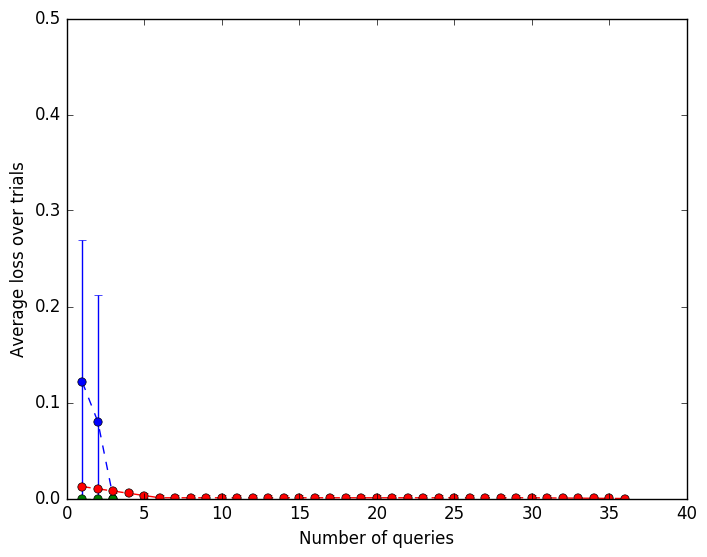
\includegraphics[width=12em]{figure_synthetic_2_uniform} &
        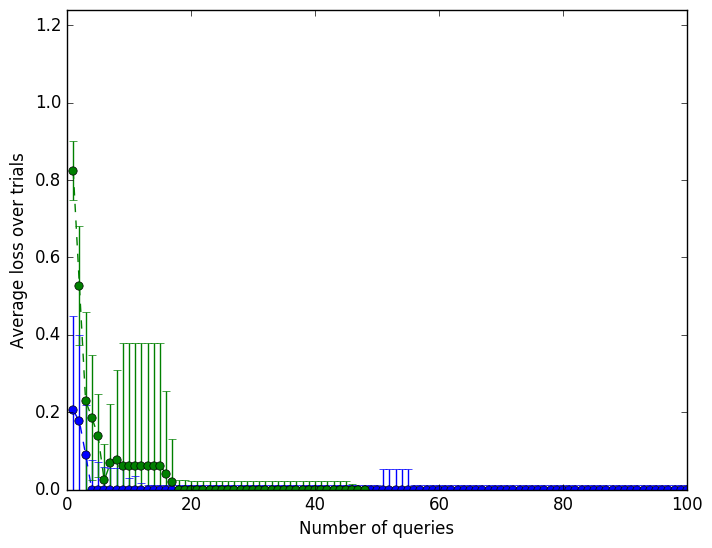
\includegraphics[width=12em]{figure_synthetic_3_uniform} &
        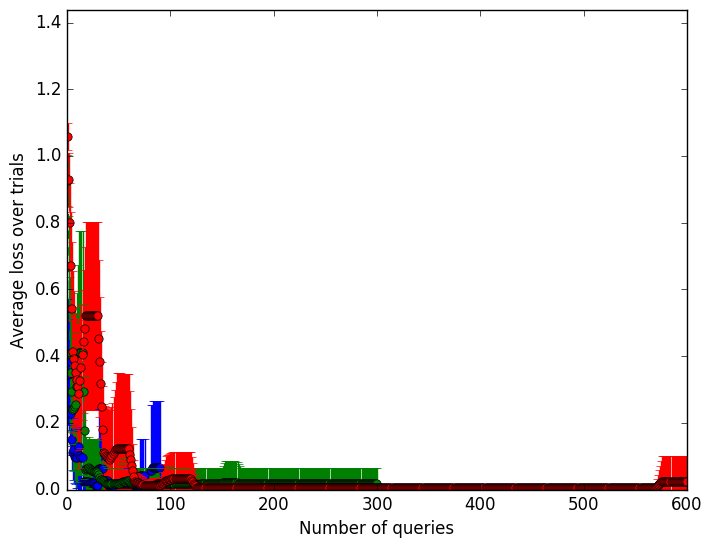
\includegraphics[width=12em]{figure_synthetic_4_uniform} &
        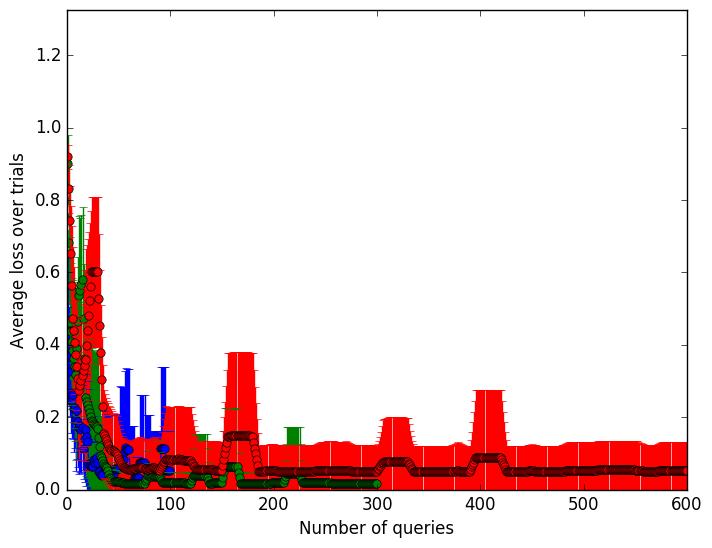
\includegraphics[width=12em]{figure_synthetic_5_uniform}
        \\
        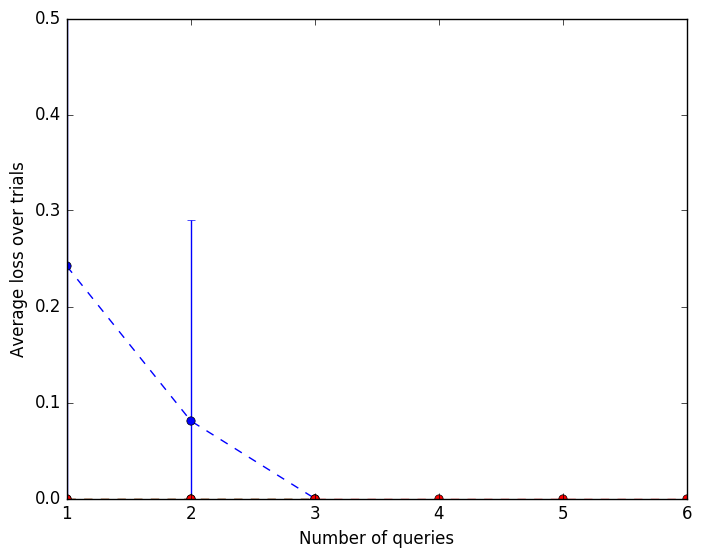
\includegraphics[width=12em]{figure_synthetic_2_uniform_sparse} &
        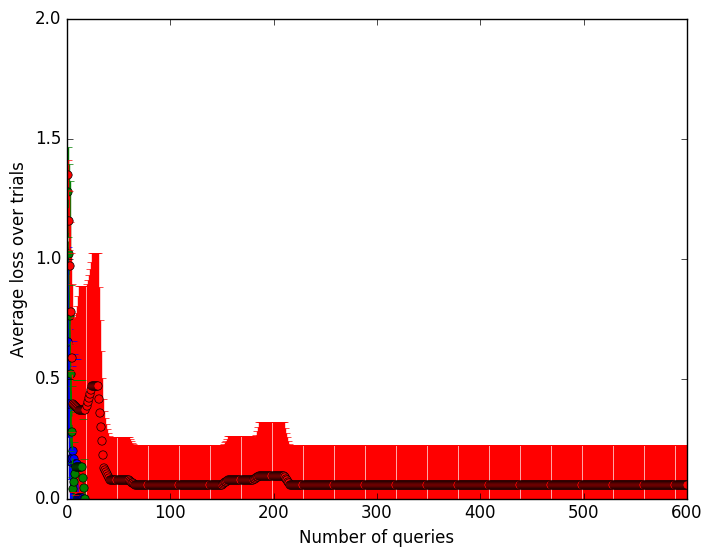
\includegraphics[width=12em]{figure_synthetic_3_uniform_sparse} &
        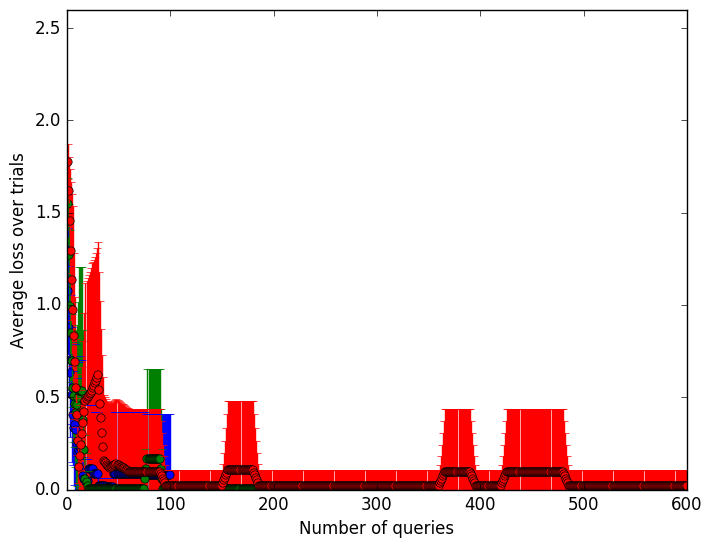
\includegraphics[width=12em]{figure_synthetic_4_uniform_sparse} &
        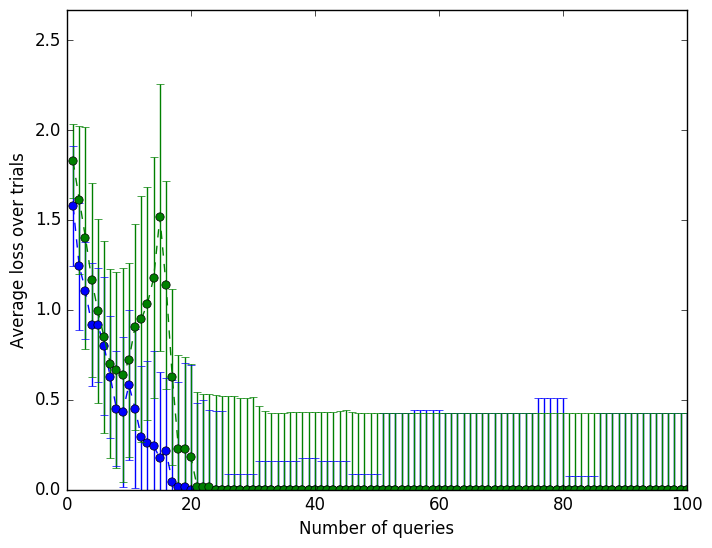
\includegraphics[width=12em]{figure_synthetic_5_uniform_sparse}
        \\
        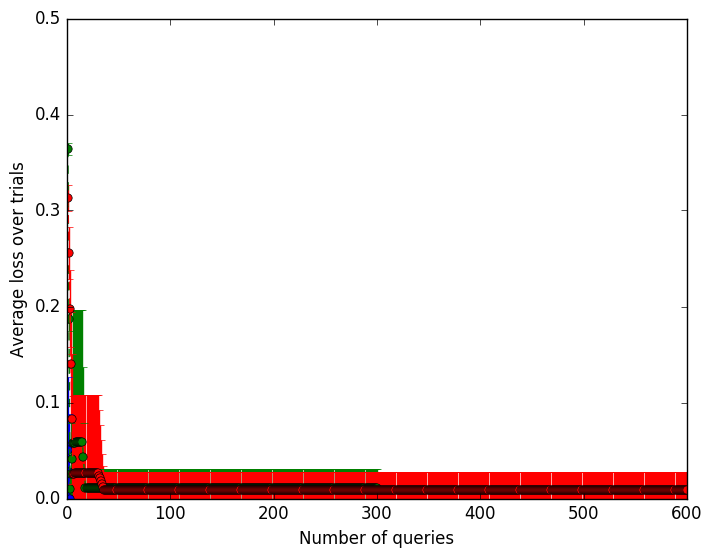
\includegraphics[width=12em]{figure_synthetic_2_normal} &
        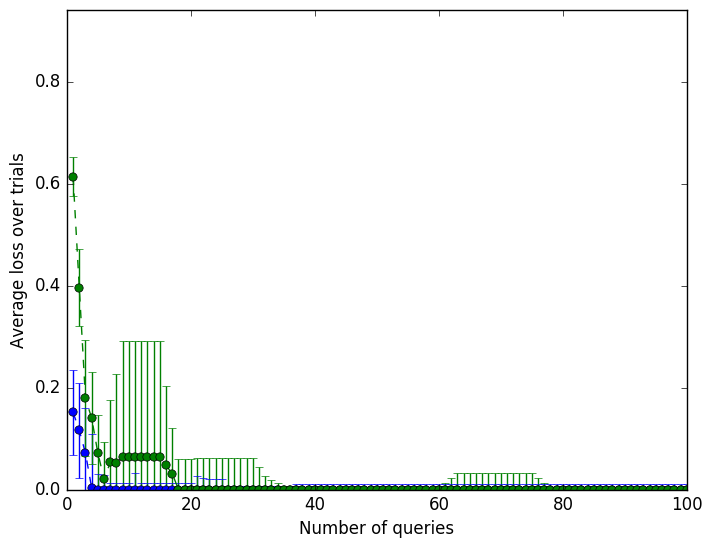
\includegraphics[width=12em]{figure_synthetic_3_normal} &
        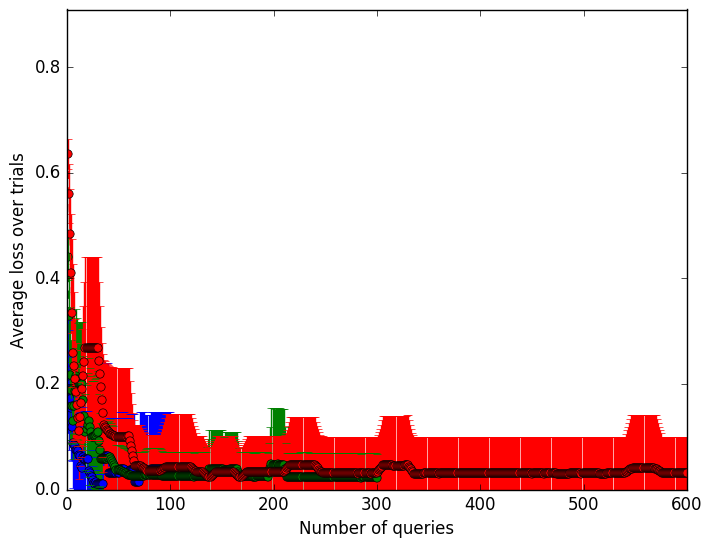
\includegraphics[width=12em]{figure_synthetic_4_normal} &
        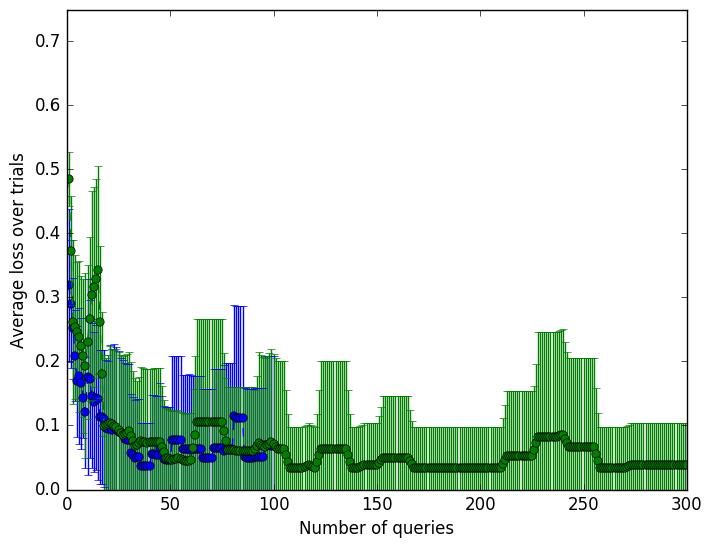
\includegraphics[width=12em]{figure_synthetic_5_normal}
        \\
        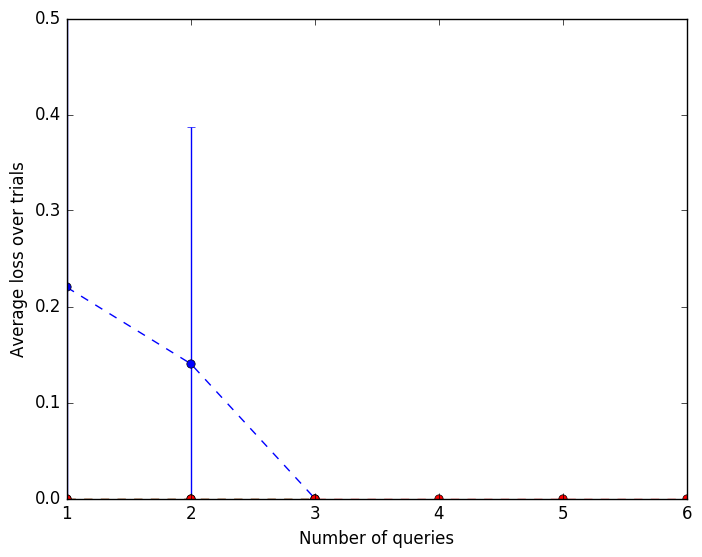
\includegraphics[width=12em]{figure_synthetic_2_normal_sparse} &
        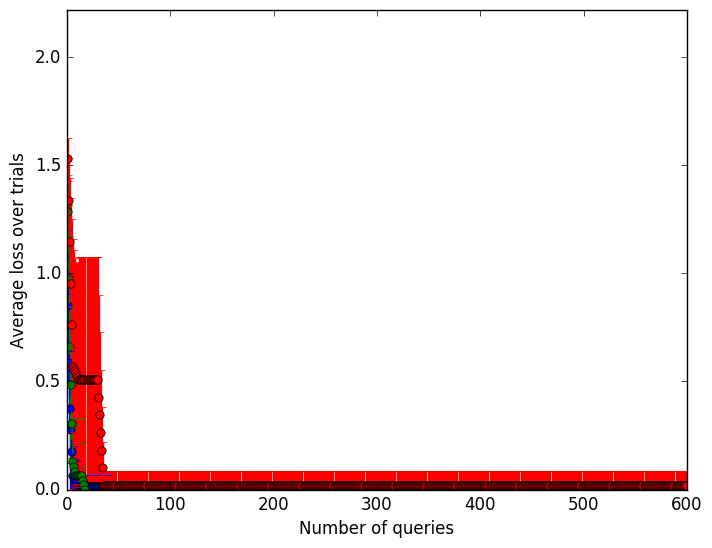
\includegraphics[width=12em]{figure_synthetic_3_normal_sparse} &
        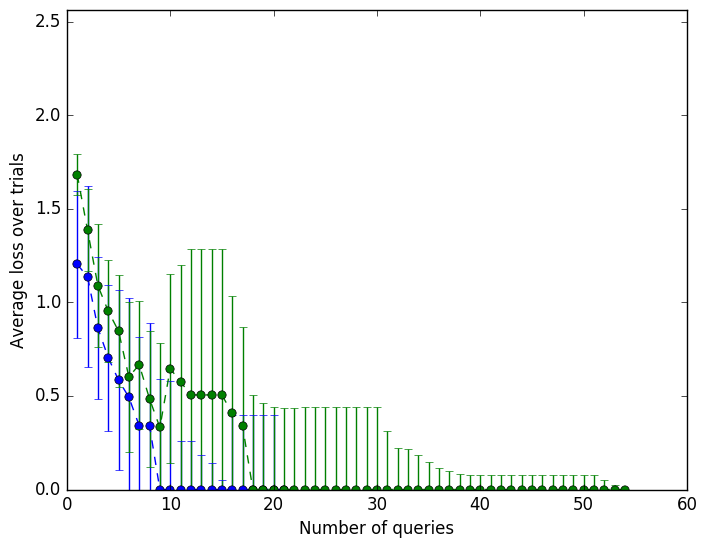
\includegraphics[width=12em]{figure_synthetic_4_normal_sparse} &
        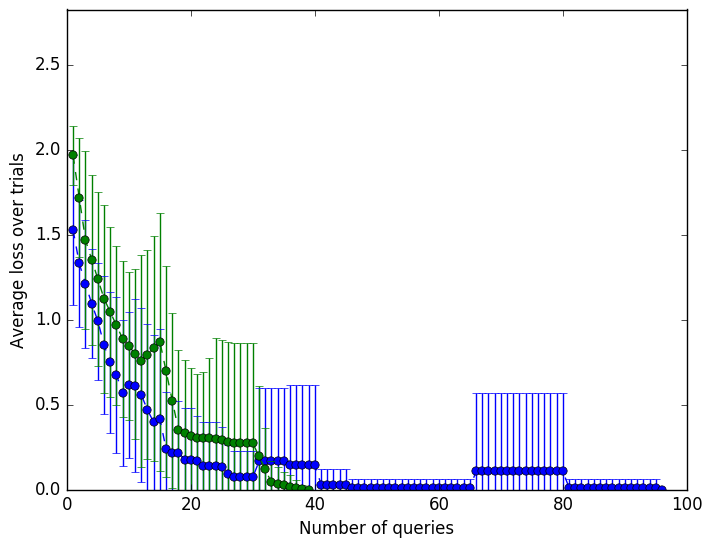
\includegraphics[width=12em]{figure_synthetic_5_normal_sparse}
    \end{tabular}
    \caption{Results on the synthetic dataset. Each row represents a different
    setting: uniform, uniform sparse, normal, normal sparse. Color indicates
    the set size $k$: blue means $k=2$, greed $k=3$, and red $k=4$.}
\end{figure}

\twocolumn

\end{document}
